\chapter{Fundamentação Teórica e Revisão Bibliográfica}
\label{sec:Referencial}

Este capítulo trata das bases teóricas necessárias para este trabalho. Ele é dividido em três seções, cada um abordando um assunto considerado essencial para o entendimento do leitor.

A primeira sessão apresenta conceitos básicos sobre FPGAs, o que são, para que servem e como programá-los, com uma pequena explicação sobre as principais linguagens de descrição de hardware.

A segunda fala sobre osciladores em anel, explica seu funcionamento e mostra, com exemplos práticos, porque é uma topologia muito utilizada em ensaios de circuitos CMOS.

Já a terceira apresentar os efeitos de envelhecimento que afetam circuitos, focando no NBTI, que vem se tornando o principal componente na degradação da vida útil dos dispositivos.

\section{FPGAs}

FPGA, ou \textit{Field Programmable Gate Arrays}, são dispositivos eletrônicos que são baseados em matrizes de blocos lógicos configuráveis que são conectados via interconexões programáveis \cite{AmdFpga}. Eles podem ser programados e reprogramados para as funcionalidades desejadas.

Sua utilização é necessária em aplicações onde uma implementação em \textit{software} utilizando um microcontrolador não é capaz de cumprir os requisitos de frequência de operação \cite{Sulaiman}.

O que cada bloco lógico possui internamente depende da fabricante e modelo do dispositivo, mas de forma geral possuem pelo menos \textit{Look-Up Tables} (LUTs), que são implementações em hardware de tabelas verdade e elementos de memória, como Flip-Flops \cite{Sato}.

A Figura \ref{fig:FPGAStructure} ilustra a estrutura básica de um FPGA mostrando os blocos lógicos configuráveis, as conexões programáveis.

\begin{figure}[H]
    \centering
    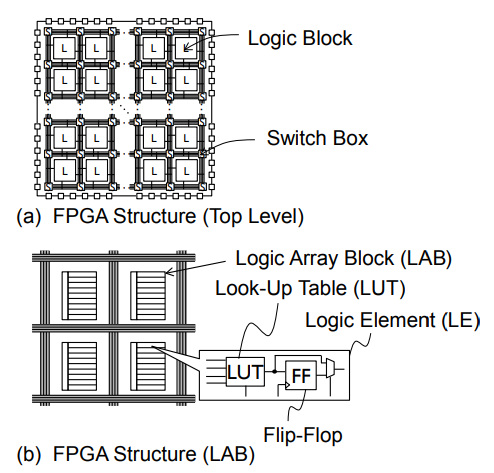
\includegraphics[scale=0.5]{figures/ReferencialTeorico/FPGAStructure.png}
    \caption{Estrutura de um FPGA. Fonte: \cite{Sato}}
    \label{fig:FPGAStructure}
\end{figure}

Os FPGAs são, de forma geral, programados utilizando linguagens de descrição de \textit{hardware} (HDL), sendo VHDL e Verilog as mais utilizadas \cite{Ain}. Essas linguagens, diferentemente de linguagens de programação convencionais onde se escreve uma série de comandos que serão executados de maneira sequencial, descrevem um circuito elétrico que será sintetizado no dispositivo.

A linguagem VHDL é pode ser utilizada para modelar sistemas digitais em diversos níveis de abstração indo do nível de algoritmo ao nível de portas lógicas. A complexidade pode variar do mais simples ao mais complexo \cite{Wunnava}. A Figura \ref{fig:Vhdl} mostra que a linguagem VHDL também pode ser definida como uma combinação de linguagens quando consideramos o nível de abstração.

\begin{figure}[H]
    \centering
    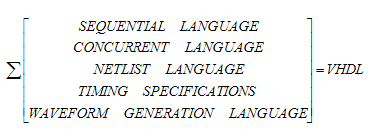
\includegraphics[scale=0.8]{figures/ReferencialTeorico/Vhdl.png}
    \caption{Integração de linguagens que constituem o VHDL. Fonte: \cite{Wunnava}}
    \label{fig:Vhdl}
\end{figure}

% VHDL is a hardware description language employed to model a digital system or digital hardware device at many levels of abstraction, ranging from the algorithmic level to the gate level (Bhasker, 1999a). The complexity of the digital system being modeled could vary from that of a simple gate to a complete digital electronic  system,  or  anything  in  between.  The  digital  system  can  also  be  described  hierarchically.  The VHDL language can also be described as a combination of languages as shown in Figure 1.

A linguagem Verilog permite descrever sistemas digitais desde o nível de portas lógicas ao nível de algoritmo. Também descreve um design do ponto de vista comportamental, de fluxo de dados, estrutural e de atrasos \cite{Bhasker}. Além disso, define sintaxe, semântica e estrutura para realizar simulações, facilitando os testes, em nível de simulação, antes da prototipação e possui simbologia e estrutura parecida com a linguagem C, tornando-se mais familiar para quem for utilizá-la \cite{Wunnava}.

\section{Oscilador em Anel}
O oscilador em anel é uma topologia de circuito muito utilizada para a caracterização de parâmetros de circuito de diversos tipos. Um dos principais motivos para isso é a capacidade de representar uma aplicação operando em alta velocidade. Segundo \cite{Bhushan} medidas feitas sob estas condições são mais próximas das aplicações reais da tecnologia do que parametrização dc convencionais, o que é verdade principalmente para dispositivos CMOS de alta performance.

Eles também são utilizados como sensores de alta precisão que aumentam a confiabilidade de um chip, podendo ser usado para monitorar diversos parâmetros como variações de processo, temperatura e efeitos de envelhecimento \cite{Sato}. Podem ser facilmente implementados e possuem um consumo de energia pequeno.

O circuito do oscilador em anel consiste em portas lógicas inversoras ligadas em sequência com uma realimentação entre a saída da última e a entrada da primeiro. É necessário que haja um número ímpar de inversores, para assim haver uma inversão periódica da entrada e da saída. O atraso de propagação de cada inversor e a realimentação gera uma onda quadrada na saída.

O período da oscilação é duas vezes o somatório do atraso de cada inversor. A Equação \ref{eq:TotalDelay} mostra frequência de oscilação, considerando que todos os inversores têm o mesmo atraso, onde N representa o número de inversores e Ta representa o tempo de atraso de um inversor.

\begin{equation}
    F = \frac{1}{2.N.Ta}
    \label{eq:TotalDelay}
\end{equation}
         
A Figura \ref{fig:RingOsc} mostra o diagrama do oscilador em anel. O circuito em questão também possui um sinal de \textit{enable}, que, além de servir para controlar o funcionamento do oscilador, também evita que o circuito entre em um estado de metaestabilidade e não oscile.

\begin{figure}[H]
    \centering
    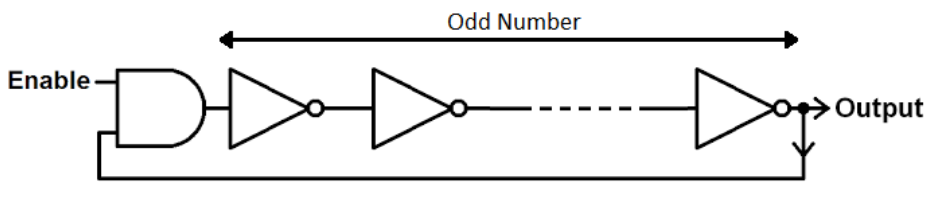
\includegraphics[width=\linewidth]{figures/ReferencialTeorico/RingOscModified.png}
    \caption{Oscilador em Anel. Fonte: \cite{Sparkfun}, modificado pelo autor}
    \label{fig:RingOsc}
\end{figure}

Uma quantidade na casa das centenas de inversores no circuito reduzirá as variações aleatórias intrínsecas de cada MOSFET que poderiam aparecer caso fossem medidos individualmente, permitindo uma caracterização mais confiável e robusta.

O trabalho de \cite{Bhushan} descreve estratégias de design para estruturas de osciladores em anel e também apresenta o uso dessas estruturas para mensurar consumo de energia e outros parâmetros de MOSFETs.

Um outro trabalho, \cite{Michal} realizou estudos para reduzir o consumo de energia de osciladores em anel, conseguindo isso reduzindo o número de inversores, mas acoplando capacitores a cada um deles para aumentar o atraso.
\section{Efeitos de Envelhecimento}
Os efeitos que causam envelhecimentos em circuitos podem ser divididos em dois grupos, os que causam falhas abruptas e os que causam deriva de parâmetros ao longo do tempo. Os principais exemplos do primeiro grupo são os TDDB (\textit{time-dependent dielectric breakdown}) e EM (\textit{electromigration}) \cite{Lorenz}. Já, para o segundo grupo, se tem o NBTI (\textit{negative bias temperature instability}) e o HCI (\textit{hot carrier injection}) \cite{Lorenz}.

Os efeitos do primeiro grupo devem ser tratados estocasticamente, já os do segundo grupo podem ser tratados deterministicamente \cite{Lorenz}.
       
Este trabalho tem como foco os efeitos de envelhecimento de longo prazo, portanto não será tratado sobre os efeitos que causam falhas abruptas.

\subsection{Bias-Temperature Instability}
\label{sec:BiasTemperatureInstability}

A variação da tensão de \textit{threshold} ($\Delta$Vth) dos transistores tipo p e tipo n é a principal característica a ser levada em conta ao analisar o envelhecimento acelerado de tecnologias CMOS. Essa variação acarreta em uma menor velocidade de chaveamento dos transistores.

Uma das principais causas da variação da tensão de \textit{threshold} é o fenômeno Bias-Temperature Instability (BTI), mais especificamente o Negative BTI (NBTI) afetando os transistores do tipo p e o Positive BTI (PBTI) afetando os transistores do tipo n.

O NBTI vem sendo estudado desde a década de 60 \cite{Alam}, mas com dispositivos CMOS de nós tecnológicos cada vez menores, esse fenômeno se torna um dos principais fatores que determinam a longevidade de transistores PMOS, diferentemente de transistores NMOS, que o principal fator é o HCI \cite{Bhardwaj}.

A miniaturização dos transistores aumenta o impacto desse efeito \cite{Banaszeski}, devido a campos elétricos maiores devido a óxidos mais finos, temperaturas maiores causadas pelo aumento na densidade de transistores e o uso de dielétricos \textit{high-k}, que estão mais propensos a apresentar falhas.

Transistores PMOS possuem uma tensão de \textit{threshold} negativa. O NBTI diminui a tensão de \textit{threshold} dos transistores PMOS, portanto, aumenta o valor absoluto dela, tornando-o ainda mais negativo.

\subsubsection{Mecanismos do NBTI}

% De acordo com \cite{Zeng} os mecanismos físicos do NBTI podem ser explicados através de três fenômenos não relacionados, que são: a geração de armadilhas na interface, o aprisionamento de lacunas e a geração de armadilhas no óxido do bulk.

O NBTI não pode ser explicado por um único mecanismo físico, mas por uma superposição de diversos processos \cite{Butzen}. Dois desses fenômenos são os mais aceitos, sendo eles: a geração de armadilhas na interface, o aprisionamento de lacunas.

O primeiro pode ser explicado pelo modelo de Reação-Difusão (RD), que diz que o NBTI é causado por ligações Si-H quebradas na interface entre o substrato e o oxido do gate. Essas ligações Si-H são formadas na fabricação do dispositivos para impedir que os átomos de silício fiquem com a valência incompleta após a colocação da camada de óxido de silício (SiO\small{2}) sobre o substrato. As ligações pendentes são denominadas estados de interface e podem voltar a ocorrer devido a campos elétricos elevados e alta temperatura \cite{Banaszeski}.

A Figura \ref{fig:PmosCrossSec} mostra as ligações Si-H na interface entre o gate e o substrato de um transistor PMOS.

\begin{figure}[H]
    \centering
    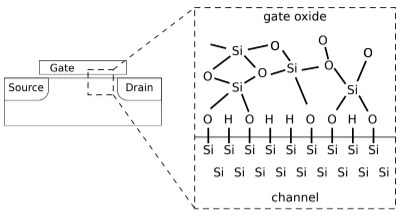
\includegraphics[scale=1]{figures/ReferencialTeorico/Cross section of a PMOS transistor.png}
    \caption{Seção da interface gate-substrato de um transistor PMOS. Fonte: \cite{Lorenz}}
    \label{fig:PmosCrossSec}
\end{figure}

Os estados de interface resultante deterioram parâmetros do transistor. Isso pode ser modelado pelo sistema RD, composto de dois processos: uma reação local e uma difusão dos produtos da reação.

A taxa de geração dessas interfaces é dada pela Equação \ref{eq:TaxaInteface} \cite{Lorenz}.

\begin{equation}
    \label{eq:TaxaInteface}
    \diff{N{\textsubscript it}}{t} = K{\scriptstyle F}(N{\scriptstyle 0} - N{\scriptstyle it}) - K{\scriptstyle R}N{\scriptstyle H}(0)N{\scriptstyle it}
\end{equation}

O primeiro termo do lado direito da equação mostra a componente de geração dos estados de interface, já o segundo termo descreve a regeneração das ligações, também denominada \textit{annealing} reverso, uma característica especial do NBTI.

$N\scriptstyle{0}$ representa a quantidade inicial de ligações Si-H, $N\scriptstyle{it}$ representa o número de estados de interface e $K\scriptstyle{R}$ é a taxa constante de criação de ligações quebradas. No termo de recuperação $N\scriptstyle{H}(0)$ representa o número de átomos de hidrogênio na interface do silício com o óxido, $K\scriptstyle{R}$ é a taxa constante de \textit{annealing} reverso das ligações incompletas e átomos de hidrogênio em ligações Si-H.

O lado direito da equação mostra que os estados de interface voltam a diminuir quando a condição de estresse, causada pela alta temperatura e o campo elétrico, é removida.

A criação de estados de interface é limitado pela difusão dos átomos de hidrogênio, como mostrado na Equação \ref{eq:TaxaDifusao}.

\begin{equation}
    \label{eq:TaxaDifusao}
    \diff{N{\scriptstyle it}}{t} = - D{\scriptstyle H}\diff{N{\scriptstyle H}}{x} + N{\scriptstyle H}\mu{\scriptstyle H}E{\scriptstyle ox}
\end{equation}

Onde $D\scriptstyle{H}$ representa o coeficiente de difusão, $\mu\scriptstyle{H}$ representa a mobilidade dos átomos de hidrogênio e $E\scriptstyle{ox}$ representa o campo elétrico que atravessa o óxido.

O segundo termo pode ser negligenciado para átomos ou moléculas eletricamente neutros \cite{Lorenz}. $K\scriptstyle{F}$, $K\scriptstyle{R}$ e $D\scriptstyle{H}$ dependem da temperatura. $K\scriptstyle{F}$ também depende do campo elétrico aplicado. Isso demonstra que as interfaces só são geradas quando um campo elétrico é aplicado, o que não é necessário para o \textit{annealing} e para a difusão.

As Equações \ref{eq:TaxaInteface} e \ref{eq:TaxaDifusao} formam um sistema que pode ser resolvido caso seja considerado que $N\scriptstyle{it}$ é muito menor que $N\scriptstyle{0}$. A Equação \ref{eq:ResultanteRD} mostra a solução desse sistema e a dependência da quantidade de interfaces com relação o tempo.

\begin{equation}
    \label{eq:ResultanteRD}
    N{\scriptstyle it} = \sqrt{\frac{K{\scriptstyle F}N{\scriptstyle 0}}{2K{\scriptstyle R}}}(D{\scriptstyle H}t)^{n}
\end{equation}

Onde n representa a constante exponencial de difusão e é sempre menor que 1, de forma que a geração das interfaces irá desacelerar com o tempo.

A variação Vth será proporcional ao $N\textsubscript{it}$, de forma que poderá ser escrito como mostrado na Equação \ref{eq:VthProp}, onde $\Phi\scriptstyle{S}$ é o potencial de superfície e $C{\scriptstyle ox}$ é a capacitância do óxido.

\begin{equation}
    \label{eq:VthProp}
    V{\scriptstyle th} \propto - \frac{qN{\scriptstyle it}(\Phi{\scriptstyle S})}{C{\scriptstyle ox}}
\end{equation}

Porém, esse fenômeno não explica completamente o fenômeno, não descrevendo corretamente a recuperação rápida que ocorre quando as condições de estresse não estão mais presentes \cite{Gilson}.

Um segundo mecanismo relacionado, denominado \textit{Trapping/Detrapping}, é baseado no aprisionamento de lacuna em defeitos no óxido pre-existentes ou provenientes de estresse elétrico \cite{Butzen}. O campo elétrico que é gerado no gate quando o PMOS está negativamente polarizado causa o tunelamento de portadores do canal, levando-as diretamente até nas falhas no óxido. Esse fenômeno vem sendo cada vez mais relevante na degradação por NBTI, considerando que falhas no óxido são mais comuns em transistores \textit{high-k}.

Cada armadilha apresenta como característica a probabilidade de capturar e liberar um portador e o valor do impacto na tensão de \textit{treshold} será gerado em caso de captura. As probabilidades tem relação com os tempos médios entre as capturas e emissões, já o impacto na tensão de \textit{treshold} tem relação com a localização em que a armadilha está localizada, podendo ser muito relevante caso obstrua o caminho de percolação do canal. 

% O modelo Trapping/Detrapping foi inicialmente desenvolvido para explicar a rápida recuperação do efeito de BTI. Assim surgiu um modelo misto, onde dois modelos coexistem: criação de defeitos na interface, dado pelo modelo Reaction-Difusion, e a captura e liberação de cargas por armadilhas pré-existentes no interior do óxido do transistor (HUARD, 2007). Neste modelo, a criação de defeitos na interface é o responsável pela parte permanente, não recuperável, da degradação enquanto as armadilhas, pré-existentes no interior do óxido, seriam responsáveis pela parte recuperável de BTI.

% Modelos mais recentes, (GRASSER, 2009) (KACZER, 2009), propõem que BTI pode ser explicado unicamente pelo efeito de captura e liberação de portadores no interior do dielétrico.

% No modelo Trapping/Detrapping, é explicada a variação de Vth pela pré-existência de armadilhas no interior do óxido, na qual cada armadilha tem como propriedades as probabilidades de captura e emissão, assim como, o desvio que causará no Vth. As probabilidades de captura e emissão são dadas pelo de tempo de captura e pelo tempo de emissão, que são os tempos médios transcorridos para que a armadilha capture um portador e emita esse portador, respectivamente. Esses tempos são log-uniformimente distribuídos, ou seja, armadilhas com diversas ordens de grandezas diferentes podem ser encontradas com a mesma probabilidade no óxido do transistor (GRASSER, 2010).

% De acordo com o modelo, quando uma armadilha é ocupada por um portador de carga (elétron ou lacuna) ela ficará eletricamente carregada. Assim, a tensão de limiar do transistor é alterada, de acordo com a localização da armadilha nas três dimensões do óxido (espessura, largura e comprimento). A localização na espessura do óxido determina o efeito eletrostático que a armadilha terá na porta e no canal de inversão do transistor, já a posição da armadilha na largura e no comprimento do óxido poderá determinar quão impactante será seu efeito na mobilidade dos portadores no transistor, já que o seu efeito eletrostático pode obstruir um caminho de percolação, ou percolation-path, no canal (KACZER, 2010) (Ver Seção 2.5), diminuindo drasticamente a sua condutividade. A localização da armadilha no comprimento do canal também determina o impacto da armadilha na tensão superficial ao longo da fonte e do dreno. Combinando todos os efeitos, dados pela localização da armadilha no canal, tem-se o desvio no Vth dado por uma determinada armadilha.

% Durante o período de estresse, armadilhas com diferentes tempos de captura e diferentes desvios de Vth são povoadas, alterando assim, a tensão limiar ao longo do tempo, conforme ilustrado na Figura 2.7, a seguir.


% Transistors with high-κ dielectric have higher density of pre-existing defects. From this point-of-view, hole trapping/detrapping is becoming the dominant contributor to NBTI degradation (KACZER, 2010).

Caminhos de percolação são os caminhos de condução que se formam em transistores nanométricos nos lugares onde há a falta de átomos dopantes, pois estes formam barreiras onde a energia de condução é maior, bloqueando os portadores \cite{Banaszeski}.

% É sabido que a região onde se encontra o átomo dopante é uma região de maior resistência para a passagem do portador, funcionando como barreiras onde a energia de condução é mais elevada. Assim, em transistores nanométricos, onde não há presença de dopantes formam-se caminhos definidos pelo qual ocorre a condução da corrente, chamados de caminho de percolação, ou percolation-path (ASHRAF, 2011).

Esses dois mecanismos podem sem considerados simultaneamente, sendo o primeiro responsável por uma componente permanente da degradação e o segundo responsável por uma componente recuperável da degradação \cite{Banaszeski}.

Cada um desses fenômenos contribui para a variação da tensão de treashold resultando na Equação \ref{eq:SomaVth}. Onde $V\scriptstyle{IT}$ á a contribuição das armadilhas na interface (primeiro mecanismo), $V\scriptstyle{HT}$ é a contribuição do aprisionamento em defeitos pré existentes e $V\scriptstyle{OT}$ é a contribuição do aprisionamento em defeitos gerados eletricamente (segundo mecanismo).

\begin{equation}
    \label{eq:SomaVth}
    \Delta V{\scriptstyle {th}} = \Delta V{\scriptstyle {IT}} + \Delta V{\scriptstyle {HT}} + \Delta V{\scriptstyle {OT}}
\end{equation}

A Equação \ref{eq:VthTempo} mostra uma aproximação da variação da tensão de treshold ao longo do tempo considerando um nó tecnológico específico e um certo conjunto de condições ambientais \cite{Butzen}.

\begin{equation}
    \label{eq:VthTempo}
    \Delta Vth = A(TSP.t)^n
\end{equation}

Onde A é uma constante que depende da tecnologia, t é o tempo, n é a constante exponencial do NBTI e TSP é a probabilidade do transistor estar negativamente polarizado.

O TSP de um transistor pode depender não só de seu duty cicle, mas também de sua posição na topologia do circuito. Por exemplo, no caso de dois transistores que compõe a malha de pull-up de uma porta NOR, o TSP do transistor superior depende apenas de seu sinal de entrada, já o TSP do inferior depende da combinação de seu sinal de entrada e do sinal de entrada do transistor superior, de forma que o transistor superior terá uma tendência maior a sofrer envelhecimento.

Quando não há campo elétrico atravessando o óxido do transistor, o que no caso dos PMOS ocorre quando a tensão de gate é positiva, há a recuperação das armadilhas de interface \cite{Chen}. Ou seja, em um circuito em que um transistor alterna entre fechado e aberto, haverá uma certa recuperação da degradação quando o transistor estiver fechado. A Figura \ref{fig:recover} exemplifica esse comportamento de estresse e relaxamento em um transistor.

\begin{figure}[H]
    \centering
    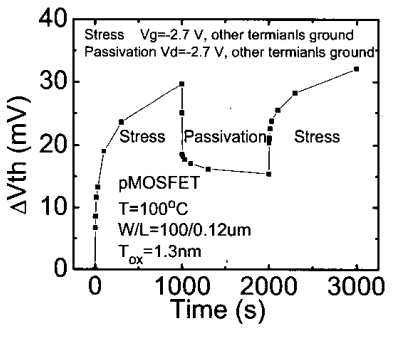
\includegraphics[scale=0.8]{figures/ReferencialTeorico/Recover.png}
    \caption{Estresse e relaxamento de um transistor. Fonte: \cite{Chen}}
    \label{fig:recover}
\end{figure}

\subsubsection{Gerando e Medindo NBTI}
\label{sec:GerandoNbti}

Muitos estudos já foram realizados para determinar em que condições o NBTI ocorre com mais facilidade em circuitos CMOS.

O fenômeno NBTI normalmente ocorre em transistores do tipo p operando com tensão de gate negativa em temperaturas variando de 100ºC a 250ºC \cite{Davidovic}. Os campos elétricos devem ser na faixa dos 6MV/cm, valores encontrados durante o \textit{burn-in} do componente, porém com transistores cada vez menores, esses campos podem ocorrer durante a operação normal de dispositivos de alta performance \cite{Schroder}. A Figura \ref{fig:CampoEletricoAno} mostra o aumento do campo elétrico que atravessa o óxido em transistores CMOS ao longo dos anos.

\begin{figure}[H]
    \centering
    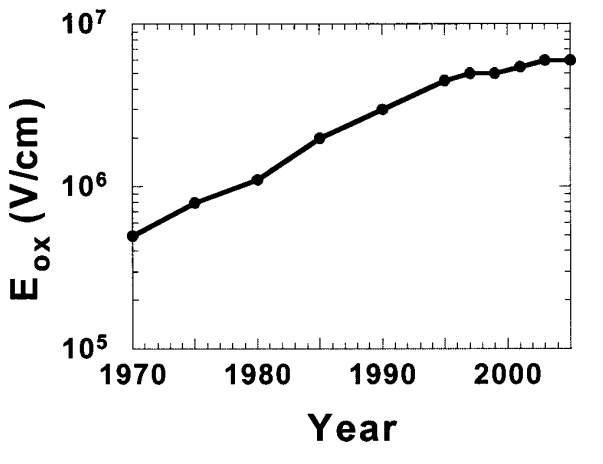
\includegraphics[scale=0.5]{figures/ReferencialTeorico/CampoEletricoAno.png}
    \caption{Campo elétrico no óxido em dispositivos CMOS ao longo dos anos. Fonte: \cite{Schroder}}
    \label{fig:CampoEletricoAno}
\end{figure}

% Typical stress temperatures lie in the 100– 250 °C range with oxide electric fields typically below 6 MV/cm, i.e., fields below those that lead to hot carrier degradation. Such fields and temperatures are typically encountered during burn in, but are also approached in highperformance ICs during routine operation.

Para aplicar o efeito de NBTI no dispositivo ensaiado no trabalho \cite{Davidovic}, os pesquisadores o estressaram por 2000 horas, aplicando tensões negativas de 30 a 45V no gate (com fonte e dreno aterrados) em uma temperatura de variando de 125 a 175ºC.

O trabalho de \cite{Bhardwaj} desenvolveu um modelo preditivo para NBTI em dispositivos CMOS de nó tecnológico de 45nm, que alcançou estimativas precisas da degradação em longo prazo da tensão de \textit{threshold} de transistores PMOS devido ao fenômeno.

Um outro trabalho \cite{Grossi}, realizou simulações para analisar os efeitos do BTI em amplificadores operacionais, e viu que o ganho DC, a frequência de corte e o \textit{slew rate} são significativamente degradados em AMPOPs operando em malha aberta. Já para Ampops operando com realimentação negativa apenas a frequência de corte mostrou uma degradação significativa.

Alguns trabalhos, inclusive, realizaram estudos dos efeitos de NBTI em osciladores em anel. Um deles \cite{Lorenz} mostra uma degradação de 5\% com 144 horas de exposição à 125°C. Já outro \cite{Sato}, que estudou métodos para diminuir o efeito de NBTI em osciladores em anel, resultou uma degradação de 0,25\%, com 42 horas de exposição, porém à apenas 85°C. Um terceiro trabalho \cite{Linder} propõe topologias de osciladores em anel que permitem estudar em separado os efeitos do PBTI, nele foi medida um degradação de 1,8\% considerando apenas o PBTI, 2,2\% considerando apenas o NBTI e 3,9\%  considerando apenas os dois efeitos combinados tendo sido realizado um estresse de 2 horas e 47 minutos (10000 segundos) segundos à 125°C.

Esses três trabalhos avaliaram a degradação causada pelo NBTI através da diminuição da frequência de osciladores em anel. Isso é viável, pois a variação da tensão de \textit{treshold} causada pelo NBTI aumentará o tempo de propagação dos transistores dos circuitos, aumentando o período de oscilação. 

% \subsection{Hot Carrier Injection}

O fenômeno conhecido como Hot Carrier Injection (HCI) vem sendo considerado uma preocupação no funcionamento de transistores MOS desde a década de 70 e vem sendo um dos efeitos de envelecimento mais estudados desde então \cite{Butzen}.

A explicação clássica para o mecanismo físico desse efeitos é a geração de portadoras de alta energia devido a campos elétricos laterais elevados em transistores MOS quando estão no estado de saturação. Se essas portadoras ganharem energia suficiente podem ultrapassar a barreira de potencial e ser injetada no óxido do gate, causando danos na interface entre o óxido e o silício, aumentando a densidade de interfaces de estado e, consequentemente degradando parâmetros do componente, entre eles a tensão de treshold \cite{Cacho}.

O HCI causa um impacto muito maior em transistores NMOS em comparação aos transistores PMOS devido ao fato da mobilidade de portadores do tipo n ser, de forma geral, maior do que a mobilidade de portadores do tipo p \cite{Jiang}.

A Figura \ref{fig:hci} mostra Hot Carriers gerados por um alto campo elétrico lateral.

\begin{figure}[H]
    \centering
    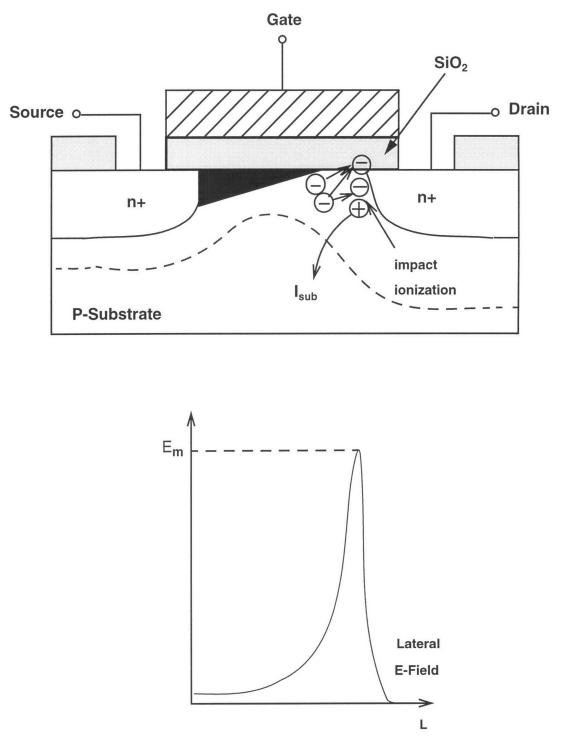
\includegraphics[scale=0.5]{figures/ReferencialTeorico/HCI.png}
    \caption{Geração de Hot Carriers (acima) devido a um campo elétrico leteral (abaixo). Fonte: \cite{Jiang}}
    \label{fig:hci}
\end{figure}


